\documentclass[../main.tex]{subfiles}

\begin{document}

\subsection{Introduction to CUDA, SGEMM, and the Naive Kernel}

\begin{frame}[fragile]
  \frametitle{What is GEMM?}
  \begin{block}{Definition: Single-precision general matrix multiplication (SGEMM)}
    \[
      C \leftarrow \alpha AB + \beta C
    \]
  \end{block}

  \pause
  \begin{itemize}
    \item Setting $\alpha=1$ and $\beta=0$ gives ordinary matrix multiplication: $C=AB$.
    \item Other values let one call scale the product and accumulate it into an existing matrix.
  \end{itemize}

  \pause
  \begin{onlyenv}<3>
    \begin{example}
      During the forward pass when training a model, we accumulate the gradients
      from the entire batch.
    \end{example}
  \end{onlyenv}

  \begin{onlyenv}<4>
    \begin{columns}
      \begin{column}{.5\linewidth}
        \begin{lstlisting}
sgemm(
  int M, int N, int K,
  float alpha, float *A, float *B,
  float beta, float *C
)
        \end{lstlisting}
      \end{column}

      \begin{column}{.5\linewidth}
        \[
          \underbrace{A}_{M\times K} \quad
          \underbrace{B}_{K\times N} \quad
          \underbrace{C}_{M\times N}
        \]

        \begin{itemize}
          \item \(M\): rows of \(A\) and \(C\)
          \item \(N\): columns of \(B\) and \(C\)
          \item \(K\): shared reduction dimension
        \end{itemize}
      \end{column}
    \end{columns}
  \end{onlyenv}

\end{frame}

\begin{frame}[fragile]
  \frametitle{CUDA Basics (Host vs. Device)}
  \begin{itemize}
    \item The CPU is known as the \textbf{host}, and manages top level logic.
    \item The GPU is known as the \textbf{device}, and does the heavy lifting.
    \item The host launches \textbf{kernels} to the device.
  \end{itemize}
  \begin{columns}
    \begin{column}{0.3\linewidth}
      \centering
      \includegraphics[width=\linewidth]{cuda_basics/basic_cuda_0.png}
    \end{column}

    \pause
    \begin{column}{0.7\linewidth}
        \begin{lstlisting}
int main() {
  const int M = 128, N = 128, K = 128;

  float *dA, *dB, *dC;
  cudaMalloc(&dA, M * K * sizeof(float);
  cudaMalloc(&dB, K * N * sizeof(float));
  cudaMalloc(&dC, M * N * sizeof(float));

  // load values into these device pointers...

  run_sgemm_naive(M, N, K, 1, dA, dB, 0, dC);

  cudaFree(dA); cudaFree(dB); cudaFree(dC);
}
        \end{lstlisting}
    \end{column}
  \end{columns}
\end{frame}

\begin{frame}[fragile]
  \frametitle{CUDA Basics (Kernel Execution)}
  \begin{itemize}
    \item A kernel runs in parallel on many \textbf{threads} on the device.
    \item The number of threads the device allocates is configured by the host, when it \textbf{launches} the kernel.
  \end{itemize}
  \begin{columns}
    \begin{column}{0.3\linewidth}
      \centering
      \includegraphics[width=\linewidth]{cuda_basics/basic_cuda_1.png}
    \end{column}

    \pause
    \begin{column}{0.7\linewidth}
      % The source is formatted to 80 columns, so keep these excerpts unwrapped.
      \lstinputlisting[
        firstline=8,
        lastline=10,
        basicstyle=\ttfamily\fontsize{5}{5.8}\selectfont,
        breaklines=false,
        belowskip=0pt
      ]{../my_sgemm/src/sgemm.cu}
        \begin{lstlisting}[
          basicstyle=\ttfamily\fontsize{5}{5.8}\selectfont,
          breaklines=false,
          aboveskip=0pt,
          belowskip=0pt
        ]
  // implementation hidden for now ...
}

        \end{lstlisting}
      \lstinputlisting[
        firstline=23,
        lastline=31,
        basicstyle=\ttfamily\fontsize{5}{5.8}\selectfont,
        breaklines=false,
        aboveskip=0pt,
        belowskip=0pt
      ]{../my_sgemm/src/sgemm.cu}
    \end{column}
  \end{columns}
\end{frame}

\begin{frame}[fragile]
  \frametitle{CUDA Basics (Threads, Blocks, Grids)}
  \begin{itemize}
    \item Threads are grouped into \textbf{blocks}.
    \item The collection of blocks requested by the host is organized in a \textbf{grid}.
  \end{itemize}
  \begin{columns}
    \begin{column}{0.3\linewidth}
      \centering
      \includegraphics[width=\linewidth]{cuda_basics/thread_block_grid.png}
    \end{column}

    \begin{column}{0.7\linewidth}
      % The source is formatted to 80 columns, so keep these excerpts unwrapped.
      \lstinputlisting[
        firstline=8,
        lastline=10,
        basicstyle=\ttfamily\fontsize{5}{5.8}\selectfont,
        breaklines=false,
        belowskip=0pt
      ]{../my_sgemm/src/sgemm.cu}
        \begin{lstlisting}[
          basicstyle=\ttfamily\fontsize{5}{5.8}\selectfont,
          breaklines=false,
          aboveskip=0pt,
          belowskip=0pt
        ]
  // implementation hidden for now ...
}

        \end{lstlisting}
      \lstinputlisting[
        firstline=23,
        lastline=31,
        basicstyle=\ttfamily\fontsize{5}{5.8}\selectfont,
        breaklines=false,
        aboveskip=0pt,
        belowskip=0pt
      ]{../my_sgemm/src/sgemm.cu}
    \end{column}
  \end{columns}
\end{frame}

\begin{frame}
  \frametitle{Why Threads, Blocks, Grids?}
  \textbf{This seems complicated, why can't we just ask for $N$ threads?}
  \pause
  \begin{block}{Relation to hardware}
    This hierarchy is closely related to how the device schedules the execution.
    We will see later how to use this to optimize performance.
  \end{block}

  \pause
  \begin{alertblock}{Thread, Block, Grid hierarchy}
    Threads are grouped into blocks of constant size/shape.

    Blocks are launched as a grid.

    We choose the dimensions of the grid to control how many blocks are launched,
    and thus how many threads are launched.
  \end{alertblock}
\end{frame}

\begin{frame}
  \frametitle{Let's design a SGEMM kernel!}
  \begin{block}{Recall}
    Recall that matrix multiplication is naturally parallel, and the output
    elements of \(C\) can be computed independently in parallel.
    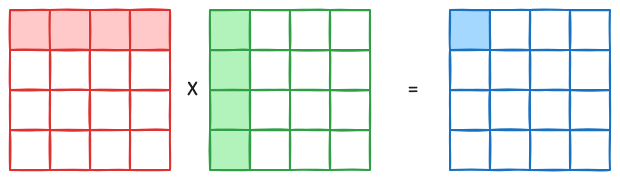
\includegraphics[width=\linewidth]{matmul.png}
  \end{block}
  \pause
  \textbf{We can naturally map one thread to each output element!}
\end{frame}

\begin{frame}[fragile]
  \frametitle{Naive SGEMM Kernel}

  \begin{columns}
    \begin{column}{0.6\linewidth}
      \lstinputlisting[
        firstline=8,
        lastline=21,
        basicstyle=\ttfamily\fontsize{6}{6.8}\selectfont,
        belowskip=0pt
      ]{../my_sgemm/src/sgemm.cu}
      \begin{lstlisting}[
        basicstyle=\ttfamily\fontsize{6}{6.8}\selectfont,
        aboveskip=0pt,
        belowskip=0pt
      ]
      \end{lstlisting}
      \lstinputlisting[
        firstline=23,
        lastline=31,
        basicstyle=\ttfamily\fontsize{6}{6.8}\selectfont,
        aboveskip=0pt
      ]{../my_sgemm/src/sgemm.cu}
    \end{column}

    \begin{column}{0.4\linewidth}
      \only<1> {
        \includegraphics[width=\linewidth]{c_matrix.png}
      }
      \only<2>{
        \includegraphics[width=\linewidth]{naive_steps/c_matrix_elem.png}
      }
      \only<3>{
        \includegraphics[width=\linewidth]{naive_steps/c_matrix_block.png}
      }
      \only<4>{
        \includegraphics[width=\linewidth]{naive_steps/c_matrix_threads.png}
      }
      \only<5>{
        \includegraphics[width=\linewidth]{naive_steps/c_matrix_indexing.png}
      }
    \end{column}
  \end{columns}
\end{frame}

\begin{frame}
  \frametitle{Naive SGEMM visualization}
  \begin{itemize}
    \item One thread computes one element of $C$.
    \item It walks one row of $A$ and one column of $B$ for the full dot product.
  \end{itemize}

  \vfill
  \centering
  \href{https://drive.google.com/file/d/1syBjMjUAfI6j8BJUSxS6mShZgX6hqguf/view?usp=sharing}{\beamerbutton{Play naive-kernel visualization}}
  \vfill
\end{frame}

\begin{frame}{Naive CUDA is already faster than the CPU}
  \centering
  \includegraphics[width=0.7\textwidth]{generated/cpu_naive_latency.png}
\end{frame}

\end{document}
